\documentclass[oneside,12pt,a4paper]{book}	

% ---------------------------------------------------
% Preambulum
% ---------------------------------------------------

\usepackage[magyar,english]{babel}
\usepackage[utf8]{inputenc}
\usepackage{t1enc}
\usepackage{indentfirst}
\usepackage{graphicx}
\usepackage{amsmath}
\usepackage{amsfonts}
\usepackage{url}
\usepackage{algorithmic}
\usepackage{algorithm}
\usepackage{mdwlist}
\usepackage{listings}
\usepackage{wrapfig}
\usepackage{epigraph}
\usepackage{placeins}
\lstset{basicstyle=\footnotesize\ttfamily}
\newcommand{\inlinecode}{\texttt}
\DeclareGraphicsExtensions{.png,.jpg}
\usepackage[left=3.5cm,right=2.5cm,top=2.5cm,bottom=2.5cm]{geometry}
\linespread{1.3}

\usepackage{tikz}

\newcounter{treeline}

\newcommand{\treeroot}[1]{% Title
\node[above] at (0,0) {#1};%
\setcounter{treeline}{0}
}

\newcommand{\treeentry}[2]{% Title, Level
\draw[->] (#2-1,-\value{treeline}/2) -- (#2-1,-\value{treeline}/2-0.5) -- (#2+0.5,-\value{treeline}/2-0.5) node[right] {#1};
\stepcounter{treeline}
}

\newcommand{\altentry}[2]{% Title, Level
\draw[->] (#2-1,-\value{treeline}/2) -- (#2-1,-\value{treeline}/2-0.5) -- (#2+0.5,-\value{treeline}/2-0.5) node[right] {#1};
\foreach \x in {1,...,#2}
{   \draw (\x-1,-\value{treeline}/2) -- (\x-1,-\value{treeline}/2-0.5);
}
\stepcounter{treeline}
}

\DeclareMathOperator{\diag}{diag}
\setcounter{secnumdepth}{3}
\setcounter{tocdepth}{3}

\begin{document}
\clearpage
\thispagestyle{empty}
\hspace{-10pt}\begin{tabular}{p{3cm} p{1cm} p{10cm}}
\raisebox{-2.5cm}{
\includegraphics[scale=0.2]{ELTE_logo}} & &
\large{\foreignlanguage{magyar}{Eötvös Loránd Tudományegyetem\newline Informatikai Kar\newline
 Programozási Nyelvek és \newline Fordítóprogramok Tanszék}}
\end{tabular}
\vspace{0.4cm}
\hrule
\vspace{6cm}
\begin{center}
\LARGE{\textbf{Applying slicing algorithms on large code bases}}
\end{center}
\vspace{3cm}
\begin{tabular}{p{7cm} p{8cm}}
\large{Tibor Brunner \vspace{5pt} \newline doktorandusz} &
\large{\foreignlanguage{magyar}{ Olivér Hechtl \vspace{5pt} \newline programtervező informatikus MSc}}
\end{tabular}\vspace{6cm}
\begin{center}
\large{Budapest, 2017}
\end{center}
\newpage
\setcounter{page}{1}
\pagenumbering{arabic}
\pagestyle{plain}
\tableofcontents

\chapter{Introduction}
\epigraph{Everyone knows that debugging is twice as hard as writing a program in the first place. So if you're as clever as you can be when you write it, how will you ever debug it?}{\textit{Brian Kernighan}}

Nowadays, there are a lot of tools available for debugging. A developer can examine call stacks, variable informations, and so on. There are a lot of times when a bug is when some variable does not behave like the writer of that code part would expect. When the programmer discovers it, he must follow back the path of assignments, and find out where did it get an unexpected value. Program slicing targets this kind of debugging. We can define a program slice as a part of the program which contains a selected statement, and all other statements which influences it, or gets influenced by it. These two types are respectively called backward and forward slicing. Basically this is what many programmers do intuitively, when facing with bugs. In this thesis, I'll introduce a few approaches for computing slices, and describe a working prototype tool application, which can analyze C++ programs, and compute slices of them. I've used the help of the Clang/LLVM compiler infrastructure, which builds the AST of the program and provides an interface to analyse it using C++.
%TODO describe the structure of the thesis.
\chapter{Slicing, methods and efficiency}
\section{About slicing}
For better understanding programs, programmers organize code into structures. They write sub-problems into functions, and organize variables and data to structs. Also, with object oriented design, they put these into classes. These are all good for separating the data, and the procedures on data. But these are not helpful when we need to examine a flow of data in the program. Slicing gets useful in this scenario. This is a program analysis technique introduced by Mark Weiser\cite{weiser84}. In his paper, he wrote: ``Program slicing is a decomposition based on data flow and control flow analysis''. We define slicing as a subset of the program, which only includes the statements which have transitive control or data dependency regarding the selected statement. 

\section{Types of slicing}
There is two different type of slicing known: static and dynamic. While dynamic slicing gets the statements which could affect the selected statement at a particular execution of the program with a fixed input, static slicing examines it statically, including all possible statements which could affect that selected statement. In this thesis, I'll focus on static slicing methods. There are two different subtypes of static slicing, backward and forward. They are indicating the relevant statements' direction from our selected statement. 

\section{Methods for slicing}
We can construct slices via various methods on different representations of the program. All of these are using some kind of graph structures, which can be traversed through for searching the transitive data dependences.

\subsection{Dependences}
Before I describe the various methods currently available for slicing, we must get to know what dependences in programs are. There are two kinds of dependences: control and data. They can be defined by the control flow graph (CFG) of the program. Given the following example:
\begin{figure}[h]
\begin{lstlisting}[language=C++]
int main(){
  int sum = 0;
  int i = sum;
  while (i < 11){
    sum += i;
    i++;
  }
}
\end{lstlisting}
\caption{Example program}
\label{fig:example_prog}
\end{figure}

\begin{wrapfigure}{r}{0.4\textwidth}
  \centering
    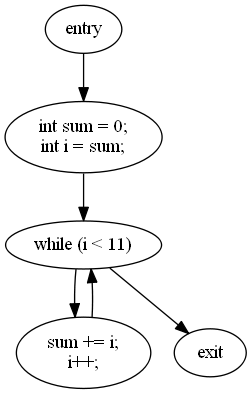
\includegraphics[width=0.38\textwidth]{horwitz_cfg.png}
  \caption{Control-flow graph}
  \label{fig:horwitz_cfg}
\end{wrapfigure}

It's control-flow graph can be seen on \ref{fig:horwitz_cfg}. This type of graph is created from the program by grouping the statements into basic blocks. Each basic block consists a maximal amount of consecutive statements without any jumps. In a high-level language, such as C++, a jump can be either a branch statement, like an \texttt{if} and a \texttt{switch-case}, or a loop statement, like a \texttt{while}. In the example, we can see that it's CFG consists three basic blocks, and two special blocks, namely \texttt{entry} and \texttt{exit}, which represent the entry and exit points of the program, respectively.

Therefore, control dependence can be defined in the knowing of post-dominance. As written in \cite{slicing-survey}:

"A node \textit{i} in th CFG is \textit{post-dominated} by a node by \textit{j} if all paths from \textit{i} to STOP pass through \textit{j}. A node \textit{j} is \textit{control dependent} on a node \textit{i} if (i) there exists a path \textit{P} from \textit{i} to \textit{j} such that \textit{j} post-dominates every node in \textit{P}, excluding \textit{i} and \textit{j}, and (ii) is not post-dominated by \textit{j}."

It basically means that every statement under a branch or loop are control dependent of the control statement's predicate. Excluding the unstructured and structured jump statements, \texttt{continue},\texttt{break} and \texttt{goto}, drawing control dependences between statements creates a tree, with the root being the inspected function, and control statements form the branches. I discuss later in detail the control dependences created by structured jumps. 

A data dependence between two statements means that if we change their order, the meaning of the program changes, or becomes ill-formed. There are two types of data dependences: \textit{flow dependences} and \textit{def-order dependences}. According to Horwitz\cite{horwitz-interproc}, we can define these with the following rules:

There is a flow dependence between statement s1 and s2 if:
\begin{enumerate}
  \item s1 defines variable x.
  \item s2 uses x.
  \item There is a path between s1 and s2 in program execution with no intervening definitions of x in between, and s2 can be reached by control from s1. 
\end{enumerate}

Definition in this context means a bit different than usual: it can be either an initial definition of a variable but an assignment where x is on the left side is also counts as a definition. In compiler theory, flow-dependence referred as reaching definition of a variable.

In the presence of loops, there are two further classification of flow-dependence: loop-carried and loop-independent. A flow-dependence is loop-carried if it satisfies all rules above and also:
\begin{enumerate}
  \item includes a backedge to the predicate of the loop.
  \item s1 and s2 are enclosed in the loop.
\end{enumerate}

Backedge means that there is a flow dependence between the statement and the predicate of the loop, therefore the loop uses the variable which that statement defines. In the example above, the statement \texttt{i++} is like this.

Loop-independent flow-dependences can be described as the common ones which has no backedge to the loop predicate. 

On the other hand, def-order dependence between statement s1 and s2 is different from loop-independent flow-dependences only in that s2 instead of using x, it also defines it. The other two rules stays the same. 

These definitions are used in all slicing methods, but differently. I will elaborate these in each section.

\subsection{Data flow equations}
\subsubsection{The algorithm}
This method is created by Mark Weiser. It is based on the analysis of the CFG. As he wrote in \cite{weiser84}, he defines a slice regarding a \textit{slicing criterion}, which consists of a pair \textit{(n, V)} where n is a statement of the program and V is a subset of the program's variables, which we are slicing on. He also writes that a slice of a program is an executable, which has only the relevant statements in it.

To calculate which statements should be included in the slice, he defines two sets of variables: \textit{directly} and \textit{indirectly relevant} variables. As written in \cite{slicing-survey}, he provides the following equations for them:

For determining \textit{directly} relevant variables and statements:
% TODO beautify

For each edge $i \rightarrow_{CFG} j$ in the CFG:
\begin{align*}
R^0_C(i) &= R^0_C(i) \cup \{ v | v \in R^0_C(j), v \notin \textsc{Def}(i) \} \cup \{ v | v \in \textsc{Ref}(i), \textsc{Def}(i) \cap R^0_C(j) \neq \emptyset \} \\
S^0_C &= \{ i | (\textsc{Def}(i) \cap R^0_C(j) \neq \emptyset, i \rightarrow_{CFG} j \}
\end{align*}

And for determining \textit{indirectly} relevant variables and statements:
\begin{align*}
B^k_C &= \{ b | \exists i \in S^k_C, i \in \textsc{Infl}(b) \} \\
R^{k+1}_C(i) &= R^k_C(i) \cup \bigcup_{b \in B^k_C} R^0_{(b, \textsc{Ref}(b))} (i) \ \\
S^{k+1}_C &= B^k_C \cup \{ \textsc{Def}(i) \cap R^{k+1}_C(j) \neq \emptyset, i \rightarrow_{CFG} j \} 
\end{align*}

He also says that a slice is statement-minimal if it couldn't have less statements. The slice then is computed in two steps:
First by determining \textit{directly} relevant variables by the equation above. In it, $\textsc{Def}(i)$ and $\textsc{Ref}(i)$ means the variables that statement $i$ defines or uses, respectively. $R^0_C(i)$ will contain the directly relevant variables of statement $i$. It starts with the values in the slicing criterion: $R^0_C(n) = V$, and for all other sets initialized as $\emptyset$. As it can be seen from the first equation above, to get the $R^0_C$ value for a node, it must use the computed values from every following node in the CFG. Weiser states in his work[1], that this is a simplification of the usual data flow information, which would use a PRE set to represent preservation of variable values. Reading the first equation, we see that variable $v$ is in the $R^0_C(i)$ set either if:
\begin{enumerate}
\item $v$ is in the slicing criterion $V$,
\item or $v$ is in \textsc{Ref}(i) and the $R^0_C$ set of the following CFG node $j$ has a value which is also in \textsc{Def}(i) 
\item or $v$ is not in \textsc{Def}(i) but $v$ is in $R^0_C(j)$.
\end{enumerate}
The last constraint ensures the propagation of the `may be used` variables through statements which does not use nor reference the variables in the slicing criterion. 

The second equation $S^0_C$ then contains the statements which are included in the slice. It goes through the CFG from start and collects all variables that may have an influence on the slicing criterion. I've listed the sets of variables which are in \textsc{Def}, \textsc{Ref} and $R^0_C$ of the statements of the example program above in the table below.

\begin{table}[h]
  \centering
  	\begin{tabular}{|l|l|l|l|}
\hline
Node                     & \textsc{Def} & \textsc{Ref}   & $R^0_C$      \\ \hline
\texttt{int sum = 0;}    & \texttt{sum} & $\emptyset$    & $\emptyset$  \\ \hline
\texttt{int i = sum;}    & \texttt{i}   & \texttt{sum}   & \texttt{sum} \\ \hline
\texttt{while (i < 11)}  & $\emptyset$  & \texttt{i}     & \texttt{i}   \\ \hline
\texttt{sum += i;}       & \texttt{sum} & \texttt{sum,i} & \texttt{i}   \\ \hline
\texttt{i++}             & \texttt{i}   & \texttt{i}     & \texttt{i}   \\ \hline
  \end{tabular}
  \caption{Results of the algorithm for the given example and criterion \texttt{(i++,\{i\})} }
  \label{tab:weiserExampleTable}
\end{table}

In this case, the set $S^0_C$ contains lines \texttt{2,3,6}. As we see, this slice is incomplete since it does not include the \texttt{while} statement. For this to be included, further iterations should be done. In the equations above, Weiser introduces the \textsc{Infl} set for every statement $i$, which consists all statements which are control dependent on $i$. In our example, it is the empty set for all statements except the \texttt{while}. Using this, he defines the $B^k_C$ set, which includes all statements which have a statement in it's \textsc{Infl} set which is included in $S^k_C$. 

Now using $B^k_C$, we can add the \texttt{while} statement since the slicing criterion is control dependent on it. This is defined in the last equation, which is almost the same as the second, but it also includes the $B^k_C$ set in it. When facing with nested branch, or looping statements, multiple levels of indirect dependences must be considered. The $R^{i+1}_C$ set contains these for each level. Because of this, Weiser's algorithm needs iterations for achieving the correct slice. The $R^k_C$ and $S^k_C$ sets are non-decreasing, and they reach a fixpoint which are called $R_C$ and $S_C$, respectively. The final $S_C$ set contains the slice for the criterion.

I must note that this method computes the \textit{backward} slice for any criterion, and cannot be used for forward slicing, since it computes only the statements which have influence on the criterion.

\subsubsection{Efficiency}
Weiser states that the complexity for computing $S_C$ is $O(n\ e\ log\ e)$. He notes that this slice is not always the smallest, since it could include statements which cannot influence the slicing variable. He shows it in the following example program:
\begin{lstlisting}
a = constant
while(p(k)){
  if (q(c)){
    b = a;
    x = 1;
  }else{
  	c = b;
  	y = 2;
  }
  k++;
}
z = x + y;
write(z)
\end{lstlisting}

For criterion \texttt{C = (write(z),\{z\})}, the set $S_C$ will contain the first statement, but it does not have an influence on \texttt{z} since on any path by which \texttt{a} can influence \texttt{c} will execute \texttt{x = 1} and \texttt{y = 2}, therefore \texttt{z} becomes a constant value in this case. 

However, computing slices with Weiser's algorithm needs little information from the program, since it requires only the CFG and the \textsc{Ref} and \textsc{Def} sets for every statement.
The downside is that it only computes backwards slices, and since the criterion is fixed, it needs to compute every set in the equations if we need a slice for a different slicing criterion of the program.

\subsection{Information flow relations}
\subsubsection{The algorithm}
This algorithm is created by Bergeretti and Carré\cite{information-flow}. It has a different approach than Weiser's: it associates the program's statements with relations: that which expression may affect which variable. These relations has the definitions in the table below.
\clearpage
\begin{table}[t]
  \centering
  	\begin{tabular}{l}
Empty statements                                                                            \\
$D_S = \emptyset$                                                                           \\
$\lambda_S = \emptyset$                                                                     \\
$\rho_S = \iota$                                                                            \\
$P_S = V$                                                                                   \\
$\mu_S = \emptyset$                                                                         \\
\hline                                                                                      
Assignment Statements, in a form of \texttt{v = e}                                          \\
$D_S = \{v\}$                                                                               \\
$\lambda_S = \Gamma(e) \times \{e\}$                                                        \\
$\rho_S = \Gamma(e) \times \{v\} \cup (\iota - \{(v,v)\})$                                   \\
$P_S = V - \{v\}$                                                                           \\
$\mu_S = \{(e,v)\}$                                                                         \\
\hline                                                                                      
Sequences of statements, in a form of A;B                                                   \\
$D_S = D_A \cup D_B$                                                                        \\
$\lambda_S = \lambda_A \cup \rho_A\lambda_B$                                                \\
$\rho_S = \rho_A\rho_B$                                                                     \\
$P_S = P_A \cap P_B$                                                                        \\
$\mu_S = \mu_A\rho_B \cup \mu_B$                                                            \\
\hline                                                                                      
Conditional statements, in a form: \texttt{if (\textit{e}) A else B}                        \\
$D_S = D_A \cup D_B$                                                                        \\
$\lambda_S = (\Gamma(e) \times \{e\}) \cup \lambda_A \cup \lambda_B$                        \\
$\rho_S = (\Gamma(e) \times (D_A \cup D_B)) \cup \rho_A \cup \rho_B$                        \\
$P_S = P_A \cup P_B$                                                                        \\
$\mu_S = (\{e\} \times (D_A \cup D_B)) \cup \mu_A \cup \mu_B$                               \\
\hline                                                                                      
Conditional statements, without else: \texttt{if (\textit{e}) A}                            \\
$D_S = D_A$                                                                                 \\
$\lambda_S = (\Gamma(e) \times \{e\}) \cup \lambda_A$                                       \\
$\rho_S = (\Gamma(e) \times D_A) \cup \rho_A \cup \iota$                                    \\
$P_S = V$                                                                                   \\
$\mu_S = (\{e\} \times D_A) \cup \mu_A$                                                     \\
\hline                                                                                      
Repetitive statements, in a form: \texttt{while (\textit{e}) A}                             \\
$D_S = D_A$                                                                                 \\
$\lambda_S = \rho^*_A((\Gamma(e) \times \{e\}) \cup \lambda_A)$                   \\
$\rho_S = \rho^*_A((\Gamma(e) \times D_A) \cup \iota)$                            \\
$P_S = V$                                                                                   \\
$\mu_S = (\{e\} \times D_A) \cup \mu_A\rho^*_A((\Gamma(e) \times D_A) \cup \iota)$\\
  \end{tabular}
  \caption{Table of information flow relations}
  \label{tab:informationFlowTable}
\end{table}
\FloatBarrier
The statements are classified into two primitive types: Empty and Assignment, and three hiearchical types: Sequence, Conditional with \texttt{else} branch, without \texttt{else} and the Repetitive statements. They are constructed from the control-flow graph. For analysis, they define \textit{variables} and \textit{expressions}.For Assignment, it's left side is the variable, and it's right side is the expression associated with it. Only this type of statement has a variable. For Conditional and Repetitive statements their conditional expression used, and Empty and Sequence has no variable or expression. There's also the definition of $\Gamma(e)$ which consists the variables which appear in $e$. We define $E$ and $V$ which contains all of the variables and expressions of the program. In $D_S$ there are the variables which $S$ \textit{may define}. In $P_S$ are the variables which $S$ \textit{may preserve}. The `multiplication` sign which we do not write between relations is the \textit{relational composition}:
For relations $X$ and $Y$, where $X \subseteq A \times B$ and $Y \subseteq B \times C$:
\begin{equation}
XY = \{(a,d) \in A \times C | (a,b) \in X, (c,d) \in Y, b = c\}
\end{equation}

The main three binary relations are the following:
\begin{enumerate}
\item $\lambda_S$, from $V$ to $E$
\item $\mu_S$, from $E$ to $V$
\item $\rho_S$, from $V$ to $V$
\end{enumerate}

For a statement $S$, $v \in V, e \in E: v \lambda_S e$ means that `the value of $v$ on entry to $S$ \textit{may be used} in the evaluation of the expression $e$ in $S$.' Taken the following program:
\begin{figure}[h]
\begin{lstlisting}[language=C++]
void fn(int x){
  read(n);             //1
  int i = 1;           //2
  while (i <= n){      //3
    if (i \% 2 = 0) {  //4
      x = 17;          //5
    }
    else{              
      x = 18;          //6
    }
    i = i + 1;         //7
  }
  write(x);            //8
}
\end{lstlisting}
\caption{Example program 2}
\label{fig:example_prog_2}
\end{figure}

It can be seen that in case of the \texttt{while} statement, variable $n$ and the predicate of \texttt{while} is in the $\lambda_{\texttt{while}}$ relation.

Taking a look at $\mu_S$, it means that for expression $e$ and variable $v$ : $e \mu_S v$ `a value of e in $S$ \textit{may be used} in obtaining the value of the variable $v$ on exit from $S$'. Looking at our example again, for the expression of \texttt{if} statement and variable $x$, $\mu_{\texttt{if}}$ holds, since the execution of assignments to $x$ are control dependent on the \texttt{if} statement.

It is basically the dual relation of $\lambda_S$, which will be very useful in aspect of slicing.

The final relation $\rho_S$ can be constructed from $\lambda_S$,$\mu_S$ and $P_S$:
\begin{equation}
\rho_S = \lambda_S\mu_S \cup \Pi_S,\  where \ \Pi_S = \{(v,v) \in V \times V\ |\ v \in P_S\}.
\end{equation}

This combination of $\lambda_S$ and $\mu_S$ creates a relation which is for $v,w \in V$:
\begin{enumerate}
\item either the entry value of $v$ to $S$ \textit{may be used} obtaining the exit value of $w$, or
\item $v = w$, and $S$ \textit{may preserve} $v$.
\end{enumerate}

In the code above, for the \texttt{if} statement we get the \texttt{\{(i,x),(i,i),(n,n),(x,x)\}} set of pairs for it's $\rho_{\texttt{if}}$ relation, since it can be seen that variable $i$ is in the predicate, so it may be used for evaluating $x$, but also, if the predicate does not hold, then the statement preserves all three variables of the program. 

These relations are different for each type of statements.

For Empty, the sets $D_S$, $\lambda_S$ and $\mu_S$ are the empty set since it has no variable in it. $P_S$ is the whole $V$ because it does not modify any variable, therefore it preserves every variable. Also, for the $\rho_S$ relation we define the identity relation $\iota$ for variables $v \in V$:
\begin{equation}
\iota = \{(v,w) \in V \times V | v = w\}.
\end{equation}
Which means the same as the $P_S$ set.

For Assignment statements, the definitions are simple. They have the form of \texttt{v = e}, so in $D_S$, there's $v$, in $P_S$, there's every variable minus $v$, since the statement assigns the value of the expression $e$ to it. In case of $\lambda_S$, it is trivial that the variables of $e$ - denoted by $\Gamma(e)$ - may be used in evaluating $e$. Also, $\mu_S$ defines that the right-hand side effects the left-hand side of the assignment. As written above, $\rho_S$ can be expressed as:
\begin{equation}
\begin{split}
\rho_S &= \lambda_S\mu_S\ \cup\ \Pi_S\ =\ (\Gamma(e) \times {e})({(e,v)})\ \cup\ \Pi_S\ =\\
&= (\Gamma(e) \times {v})\ \cup\ \Pi_S\ =\ (\Gamma(e) \times {v})\ \cup\ (\iota\ -\ \{(v,v\})
\end{split}
\end{equation}

In Assignment, $\Pi_S$ does not contain the variable, because it is being changed.

In the case of Sequence of statements, they have no direct variable or expression associated with them. They represent the single arrow between two nodes in the CFG. So, for the sequence of statements $A;B$, the relation $e \lambda_S v$ contains either
\begin{enumerate}
\item $e$ which is in $A$ and $v \lambda_A e$ or
\item $e$ is in $B$ and there is a variable $w$ that $v \rho_A w$ and $w \lambda_B e$.
\end{enumerate}

As defined above, $\rho_A$ gets all the variables from statement $A$ which are preserved or may be used, therefore they are fitting in the definition for the sequence.

Similarly, $\mu_S$ contains pairs of $(v,e)$ which either
\begin{enumerate}
\item $e$ is in $A$ and there is a variable $w$ that $e \mu_A w$ and $w \rho_B v$ or
\item $e$ is in $B$ and $e \mu_B v$
\end{enumerate}

The duality of $\lambda_S$ and $\mu_S$ can again be seen.
For $\rho_S$, we can substitute the formulas:
\begin{equation}
\begin{split}
\rho_S\ &=\ (\lambda_A\ \cup\ \rho_A\lambda_B)(\lambda_A\ \cup\ \rho_A\lambda_B)\ \cup\ (\Pi_A\ \cap\ \Pi_B)
\end{split}
\end{equation}

For brevity, I don't follow through the substitution here. The result of it is $\rho_A\rho_B$. 
In case of a sequence of statements which has more than two statements in it, we can define it by nesting: $(((A;B);C);...)$. The ordering of parentheses are irrelevant.

For Conditional statements, there is a control dependence between it's predicate $e$ and the statements $A,B$ in them. Therefore,
$(v,e)$ is in $\lambda_S$ if
\begin{enumerate}
\item $e$ is the predicate and $v \in \Gamma(e)$
\item $e$ is in $A$ and $v \lambda_A e$ or
\item $e$ is in $B$ and $v \lambda_B e$.
\end{enumerate}
%todo more text

In case of $\mu_S$, $(v,e)$ is in the relation if:
\begin{enumerate}
\item $e$ is the predicate, and either $A$ or $B$ define $v$, or
\item $e$ is in $A$ and $e \mu_A v$ or
\item $e$ is in $B$ and $e \mu_B v$.
\end{enumerate}

With substituting $\lambda_S$ and $\mu_S$ into the formula of $\rho_S$ above, we get:
\begin{equation}
\rho_S = (\Gamma(e) \times (D_A \cup D_B)) \cup \rho_A \cup \rho_B
\end{equation}

When the Conditional statement has no \texttt{else} branch, we can substitute it with an Empty expression, gaining the simplified formulas which can be seen in table \ref{tab:informationFlowTable}.

Bergeretti in his paper states that Repetitive statements can be expressed as an infinite sequence of nested conditional  statements in a form of:
\begin{lstlisting}
if(e){
  A;
  if(e){
    A;
    ...
  }
}
\end{lstlisting}

Therefore we can get the formula of $\lambda_{\textsc{Rep}}$ if we repeatedly use $\lambda_{\textsc{Cond}}$ and $\lambda_{textsc{Seq}}$, gaining the following:
\begin{equation}
\lambda_S = \rho^*_A((\Gamma(e) \times \{e\}) \cup \lambda_A)
\end{equation}
where $\rho^*_A$ is the \textit{transitive closure} of $\rho_A$.

For any relation $R$, it's transitive closure is the fixpoint of the following set:
\begin{equation}
R^* = \bigcup_{i \in \{1,2,...\}} R^i
\end{equation}
The other two relations can be similarly derived by applying their Conditional and Sequence versions, thus getting:
\begin{equation}
\begin{split}
\rho_S &= \rho^*_A((\Gamma(e) \times D_A) \cup \iota) \\
\mu_S &= (\{e\} \times D_A) \cup \mu_A\rho^*_A((\Gamma(e) \times D_A) \cup \iota)
\end{split}
\end{equation}

For determining a slice of a program with these relations, Bergeretti describes the definition of partial statements, with the formula:
\begin{equation}
E^v_S = \{e \in E\ |\ e \mu_S v\}
\end{equation}

As it can be seen from the definition of $\mu_S$, this results in the whole slice for variable $v$, if the given statement $S$ is the `statement' of the whole program, as a Sequence of top-level statements. It also gets the \textit{expressions} which may affect the variable, and not the statements consisting it. However, using $\mu_S$, we can create formulas which effectively get the desired statements from the program. It can be seen that with the dual nature of $\mu_S$ and $\lambda_S$, they can be used for backwards slicing,and for forward slicing, respectively. 

\subsubsection{Efficiency}

This algorithm is throroughly defines the flow of data across statements, taking control dependences into account. Further extensions, like applications for \texttt{switch-case} expressions can be added by defining the relations for them, on the basis of the current ones. It needs deeper parsing than Weiser's method, for getting all the variables of the expressions, and statements. However, if we parse the program code, and collect the $D_S$, $v$,$e$, $\Gamma(e)$ sets, variables and expressions for each statement, we can compute different slices for different variables and statements after for the program. In the case of large codebases, this is an important aspect of the algorithm. 

In the presence of loops, calculating the reflexive closure takes additional time. Bergeretti states the following for the complexity of the calculation of relations: $\rho_S$ has a worst case asymptotic $O(|V|^3)$. Therefore, for all statements it is $O(|E| \times |V|^3)$. For $\lambda_S$ and $\mu_S$, it is $O(|E| \times |V|^2)$ for each statement, or $O(|E|^2 \times |V|^2)$. 
If we compare these with Weiser's, it is clear that this algorithm requires more computation for slicing the program for the first time, however Bergeretti noted that these times are not problematic in real life examples.



\subsection{Dependence graph based slicing}
\subsubsection{The algorithm}
The third algorithm is first written by Ottenstein and Ottenstein\cite{ottenstein}, and has been a base for different slicing techniques, used by Susan Horwitz\cite{horwitz-interproc}, and \cite{use-of-slicing-horwitz}, \cite{program-analysis-via-graph-reachability-reps}, \cite{slicing-with-jumps} and \cite{slicing-oop}.  

This algorithm uses the Program Dependence Graph, which is a directed graph constructed either from the control-flow graph or the abstract syntax tree \textit{(AST)} of the program. Horwitz describes this graph thoroughly in her paper\cite{horwitz-interproc}. It contains the control dependence and data dependence subgraphs. The nodes of it are the statements of the program. There is a special node called the entry node, which is considered to be before any statement in the CFG. Building the graph is done in two steps: first by creating the control dependence subgraph, then drawing the data dependence edges in it. Control dependence edges has boolean labels: they are either \texttt{true} or \texttt{false}.

There is a control dependence edge between two nodes $v_1$ and $v_2$ if:
\begin{enumerate}
\item $v_1$ is the entry node, and $v_2$ is a statement which is not under any loop or branch.
\item $v_1$ is a loop or branch statement, and $v_2$ is \textit{immediately} nested under $v_1$. If $v_1$ is a loop statement, then the label of the edge is \texttt{true}, if it is a branch statement, then if $v_2$ is under the `then` branch, the label is \texttt{true}, and \texttt{false} otherwise.
\end{enumerate}

The control dependence subgraph has similar structure as the AST. It is the direct consequence of that the usually the loop and branch statements has other statements nested in them. In \cite{efficient-pdg}, there are region nodes created for predicate of each loop or branch. In practice, I have found these unnecessary to deal with. I will later discuss it in the chapter about the implementation. 

After constructing the control dependence subgraph, data dependence edges are added. The meaning of this kind of edge between $v_1$ and $v_2$ is that if we change the order of these statements then the program may become ill-formed or the computation is changed. In the aspect of slicing, there are two main different type of edges: \textit{flow dependence} and \textit{def-order dependence}. In compiler theory, in data-flow analysis there is the `use-def' or `def-use' chain, which has similar definitions what Horwitz describes in her paper. There is a flow dependence edge between nodes $v_1$ and $v_2$ if:
\begin{enumerate}
\item $v_1$ is a node which defines variable $x$ and
\item $v_2$ uses $x$ and
\item Control can reach $v_2$ after $v_1$ in an execution path which does not contain any intervening definition of $x$.
\end{enumerate}

The third rule is easy to verify if the PDG is built using the CFG, but using the `def-use' chains, it also can be derived from the AST. 

In the case of loops, there are two further sub-types of flow dependence edges: \textit{loop-carried} and \textit{loop-independent}. In addition to the three rules above, Loop-carried edges must hold that:
\begin{enumerate}
\item The path in the third rule contains a backedge to the predicate of loop $L$ and
\item $v_1$ and $v_2$ are both part of loop $L$.
\end{enumerate}

Loop-independent edges are not keeping the first rule above, so the path does not contain a backedge to the predicate.
There is a def-order dependence edge between node $v_1$ and $v_2$ if:
\begin{enumerate}
\item $v_1$ and $v_2$ defines the same variable and
\item There is a execution path between $v_1$ and $v_2$ without any intervening definition of that variable.
\end{enumerate}
\clearpage
Taken the following example program:
\begin{figure}[h]
\lstset{numbers=left}
\begin{lstlisting}[language=C++]
int main(){
  int x = 0;
  int y = 1;
  while(x >= 0){
    if (x > 0){
      y = x; //2. use here
    }else{
      x = 3;
    }
    x = 2; //1. define here
  }
}
\end{lstlisting}
\caption{Example program 3}
\label{fig:example_prog_3}
\end{figure}

\begin{wrapfigure}{r}{0.5\textwidth}
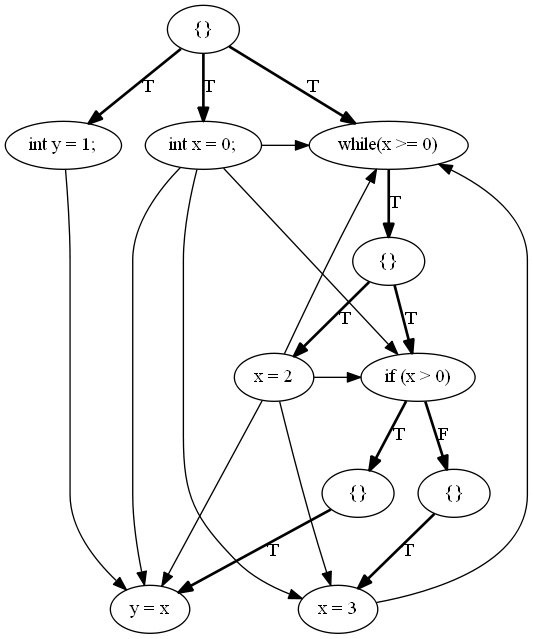
\includegraphics[width=0.5\textwidth]{loop_carried_test}
\caption{PDG of \ref{fig:example_prog_3}}
\label{fig:example_prog_3_PDG}
\end{wrapfigure}
We can see the created PDG of it on \ref{fig:example_prog_3_PDG}. The bold arrows represent the control dependence edges and the others are the data dependence edges. In her paper, Horwitz creates loop edges to the statements which are under a loop, but regarding slicing, they are not making a difference. As it can be seen, the nodes labeled \texttt{\{\}} are the brackets which consist multiple statements. I have created this example to show how a loop-carried edge can be found between different scopes under a loop statement. The comments in the example code shows the order of `def-use' relationship created by the loop: when control reaches $1.$, $x$ gets defined, then in the second second iteration control goes into the true branch of the \texttt{if} statement and reaches $2.$, creating a `def-use' data dependence between the two statements. Among this, there are examples of def-order dependence edges: between line 8. and line 10., and also between the initial definition of $x$ and other definitions later. % todo fix the graph and the definition collecting in branches.

Drawing data dependence edges are a non-trivial task. I will explain the details in the implementation chapter. However, the PDG itself when built, is a very useful abstraction of the program. To slice regarding a statement and variable in the program, we need to do only a graph reachability search in the graph over the control and data dependence edges. 
\begin{wrapfigure}{r}{0.5\textwidth}
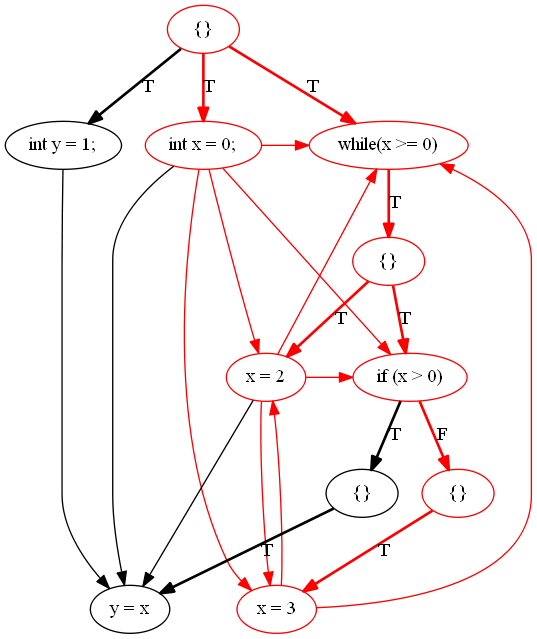
\includegraphics[width=0.5\textwidth]{loop_carried_test_backward_slice}
\caption{Backward slice of \ref{fig:example_prog_3} regarding line 9.}
\label{fig:example_prog_3_backward_slice}
\end{wrapfigure}
If we store the edges of the graph bidirectionally, the difference becomes only the direction of search between creating backward and forward slices. We can see an example of a backward slice on \ref{fig:example_prog_3_backward_slice}, regarding the $x$ variable on line 9.
% todo write more


\chapter{LLVM/Clang infrastructure}
\section{About Clang}












\section{The Clang AST}
\section{AST Matchers}

\chapter{Implementation and algorithm}
\section{The approach}
\section{Building the PDG}
\subsection{Control dependences}
\subsection{Data dependences}

\section{Implementing slicing}


\addcontentsline{toc}{chapter}{Glossary}
\begin{thebibliography}{Textttext}
\bibitem{weiser84}
  M. Weiser,
  Program slicing,
  IEEE Transactions on Software Engineering,
  10(4):352-357,
  1984.

\bibitem{slicing-survey}
  Tip, Frank,
  A survey of program slicing techniques,
  Journal of programming languages 3.3,
  121-189,
  1995. 

\bibitem{horwitz-interproc}
  Horwitz, Susan, Thomas Reps, and David Binkley,
  Interprocedural slicing using dependence graphs, 
  ACM Transactions on Programming Languages and Systems,
  (TOPLAS) 12.1: 26-60,
  1990.

\bibitem{information-flow}
  Bergeretti, Jean-Francois, and Bernard A. Carré,
  Information-flow and data-flow analysis of while-programs,
  ACM Transactions on Programming Languages and Systems,
  (TOPLAS) 7.1: 37-61,
  1985.

\bibitem{use-of-slicing-horwitz}
  Horwitz, Susan, and Thomas Reps,
  The use of program dependence graphs in software engineering,
  Proceedings of the 14th international conference on Software engineering. 
  ACM,
  1992.

\bibitem{program-analysis-via-graph-reachability-reps}
  Reps, Thomas,
  Program analysis via graph reachability,
  Information and software technology,
  40.11: 701-726,
  1998.

\bibitem{efficient-pdg}
  Harrold, Mary Jean, Brian Malloy, and Gregg Rothermel,
  Efficient construction of program dependence graphs,
  ACM SIGSOFT Software Engineering Notes,
  Vol. 18. No. 3. ACM,
  1993.

\bibitem{slicing-oop}
  Larsen, Loren, and Mary Jean Harrold,
  Slicing object-oriented software,
  Software Engineering,
  Proceedings of the 18th International Conference on. IEEE,
  1996.

\bibitem{slicing-with-jumps}
  Agrawal, Hiralal,
  On slicing programs with jump statements,
  ACM Sigplan Notices,
  Vol. 29. No. 6. ACM,
  1994.

\bibitem{ottenstein}
  Ottenstein, Karl J., and Linda M. Ottenstein,
  The program dependence graph in a software development environment,
  ACM Sigplan Notices,
  Vol. 19. No. 5. ACM,
  1984.

\end{thebibliography}

\end{document}